\section{yoghurt}
Yogurts great :)
\section{Ingredients}
\begin{itemize}
\item 1/2 gallon milk — whole or 2\% are best, but skim can also be used
\item 1/2 cup commercial yogurt containing active cultures
\end{itemize}

\section{Equipment}
\begin{itemize}
\item 3 quart or larger Dutch oven or heavy saucepan with a lid
\item Spatula
\item Instant-read or candy thermometer (one that can clip to the side of the pan)
\item Small measuring cup or small bowl
\item Whisk
\end{itemize}

\section{Method}
\begin{enumerate}
\item Heat the milk. Pour the milk into the Dutch oven and set over medium to medium-high heat. 
Warm the milk to right below boiling, about 200°F. Stir the milk gently as it heats to make sure the 
bottom doesn't scorch and the milk doesn't boil over. According to the National Center for Home Food 
Preservation, this heating step is necessary to change the protein structure in the milk so it sets as a 
solid instead of separating.

\item Cool the milk. Let the milk cool until it is just warm to the touch, 112°F to 115°F. 
Stir occasionally to prevent a skin from forming. (Though if one does form, you can either
stir it back in or pull it out for a snack!) You can help this step go faster by placing the Dutch
oven in an ice water bath and gently stirring the milk.

\item Thin the yogurt with milk. Scoop out about a cup of warm milk with a measuring cup and 
add the yogurt. Whisk until smooth and the yogurt is dissolved in the milk.

\item Whisk the thinned yogurt into the milk. Pour the thinned yogurt into the warm milk while whisking 
gently. This inoculates the milk with the yogurt culture.
\item Transfer the pot to the (turned-off) oven. Cover the Dutch oven with the lid and place the 
whole pot in a turned-off oven — turn on the oven light or wrap the pot in towels to keep the milk warm 
as it sets (ideally around 110°F, though some variance is fine). You can also make the yogurt in a dehydrator 
left at 110°F or using a yogurt maker.
\item Wait for the yogurt to set. Let the yogurt set for at least 4 hours or as long as overnight — 
the exact time will depend on the cultures used, the temperature of the yogurt, and your yogurt preferences. 
The longer yogurt sits, the thicker and more tart it becomes. If this is your first time making yogurt, start checking 
it after 4 hours and stop when it reaches a flavor and consistency you like. Avoid jostling or stirring the yogurt until 
it has fully set.
\item Cool the yogurt. Once the yogurt has set to your liking, remove it from the oven. If you see any watery whey 
on the surface of the yogurt, you can either drain this off or whisk it back into the yogurt before transferring to 
containers. Whisking also gives the yogurt a more consistent creamy texture. Transfer the to storage containers,
cover, and refrigerate. Homemade yogurt will keep for about 2 weeks in the refrigerator.
\item Your next batch of homemade yogurt. Once you start making your own yogurt, you can use some of each 
batch to culture your next batch. Just save 1/2 cup to use for this purpose. If after a few batches, you notice some 
odd flavors in your yogurt or that it's not culturing quite as quickly, that means that either some outside bacteria has 
taken up residence in your yogurt or that this strain is becoming weak. As long as this batch still tastes good to you,
it will be safe to eat, but go back to using some store-bought commercial yogurt in your next batch.
\end {enumerate}
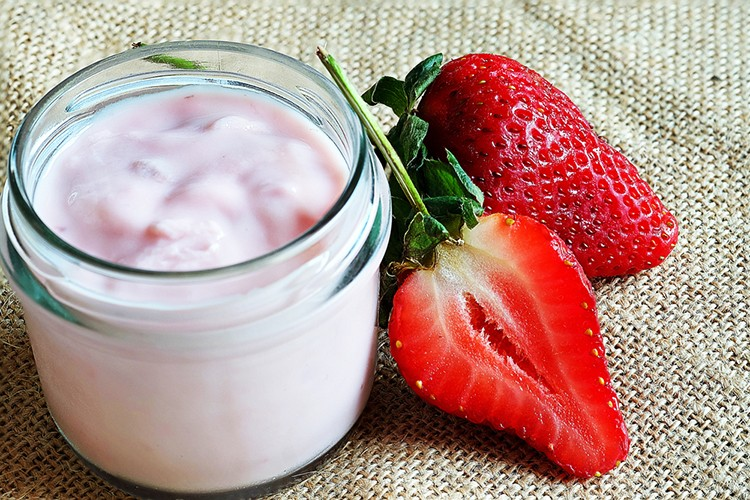
\includegraphics[scale = 0.5,natwidth=610,natheight=642]{yoghurt.jpg}


